\documentclass[12pt,pdf,hyperref={unicode}]{beamer}
%\usetheme{boxes}
\beamertemplatenavigationsymbolsempty
\setbeamertemplate{footline}[page number]
% Set it for the internal PhD thesis defence to reduce number of slides
%\setbeamersize{text margin left=0.5em, text margin right=0.5em}

\usepackage[utf8]{inputenc}
%\usepackage[english, russian]{babel}
\usepackage{bm}
\usepackage{multirow}
\usepackage{ragged2e}
\usepackage{indentfirst}
\usepackage{multicol}
\usepackage{subfig}
\usepackage{amsmath,amssymb}
\usepackage{enumerate}
\usepackage{mathtools}
\usepackage{comment}
\usepackage[all]{xy}
\usepackage{tikz}
\usetikzlibrary{positioning,arrows}
\tikzstyle{name} = [parameters]
\definecolor{name}{rgb}{0.5,0.5,0.5}

%\usepackage{caption}
%\captionsetup{skip=0pt,belowskip=0pt}

%\newtheorem{theorem}{Theorem}
%\newtheorem{statement}{Statement}
%\newtheorem{definition}{Definition}

% colors
\definecolor{darkgreen}{rgb}{0.0, 0.2, 0.13}
\definecolor{darkcyan}{rgb}{0.0, 0.55, 0.55}
%\AtBeginEnvironment{figure}{\setcounter{subfigure}{0}}
%\captionsetup[subfloat]{labelformat=empty}

%----------------------------------------------------------------------------------------------------------

\title{ Put the title of your thesis \\ here}
%\author{Name Surname}
%\institute[]{}
%\date{2024}

%---------------------------------------------------------------------------------------------------------
\begin{document}
%\begin{frame}
%\titlepage
%\end{frame}
\setcounter{page}{2}%remove here for the title
%----------------------------------------------------------------------------------------------------------
%\section{Please do not use sectioning in the presentations}
\begin{frame}{Put your title or a main part of it  here}
Couple of motivational sentences
\begin{block}{The problem}
to investigate \ldots 
\end{block}
\begin{block}{The method needs a proper name here}
put the brief idea here
\end{block}
\begin{block}{The solution} your results appears twice, as a promise here and as a contribution later
\begin{enumerate}[1)]
\item set \ldots,
\item put \ldots,
\item get \ldots.
\end{enumerate}
\end{block}
\end{frame}
%----------------------------------------------------------------------------------------------------------
\begin{frame}{Graphical highlights  as a form of your message%
\footnote{\textit{V.\,V.~Strijov et al.}  Analytic and stochastic methods of structure parameter estimation~// Informatica, 2016.}}
What the audience sees on the figure.
\begin{columns}
\begin{column}{0.3\textwidth}
\begin{enumerate}[1)]
    \item The notation and 
    \item the subjects.
\end{enumerate}
\end{column}
\begin{column}{0.7\textwidth}
	\includegraphics[width=1\textwidth]{Name-Step-3-fig}      
\end{column}
\end{columns}
\bigskip\documentclass[tikz,border=5pt]{standalone}
\usepackage{tikz}
\usetikzlibrary{shapes, arrows.meta, positioning, fit}
\usepackage{graphicx}
What are the consequences?
\end{frame}


\begin{frame}{LLMs consistency in personality scoring}
Experiment pipeline
	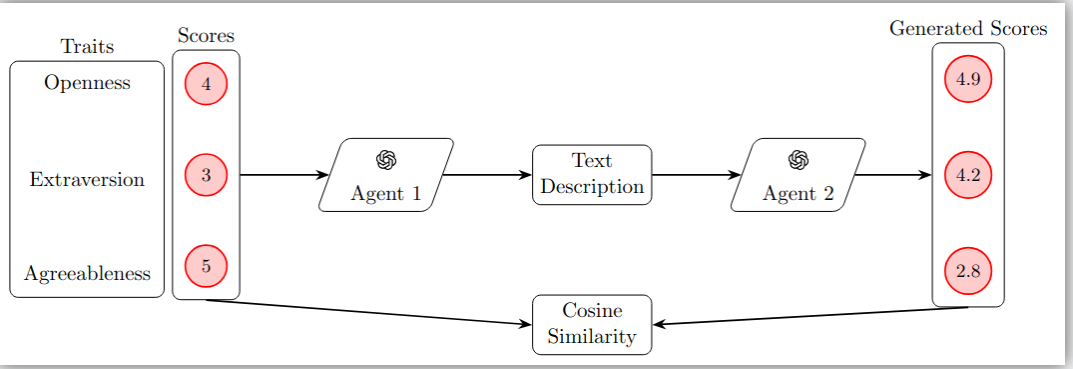
\includegraphics[width=1\textwidth]{Screenshot from 2025-03-27 01-49-06.png}  

\begin{enumerate}[1.]
    \item Big Five -- set of personality traits with a lot of research
    \item Personality conditioning -- prompting model with a personality
\end{enumerate}

     $S_{agent, traits}:$ score $\rightarrow$ text $ \ \ \ \ \ \ \ \ $$S_{agent, traits}^{-1}:$ text $\rightarrow$ score
    
\begin{center}
\textbf{Research question: $S(S^{-1}) = I$?}
\end{center}

\end{frame}


\end{document}